\chapter{Algoritmo}\label{cap.algoritmo}%Despegue, b\'usqueda y aterrizaje

\hspace{1cm} A lo largo de este cap\'itulo voy a contar las distintas fases por las que se ha pasado hasta llegar al algoritmo final. Se va a poder ver como se han producido diversos cambios a lo largo del proyecto. Esto se debe a que debido a las pruebas que se iban realizando, ve\'iamos los fallos e imperfecciones y trat\'abamos de arreglarlos. Adem\'as, seg\'un el punto en el que nos encontraramos nos inter\'esaba mas fijarnos en unos u otros detalles, por lo que no solo hab\'ia cambios en la base del algoritmo principal sino tambi\'en en el GUI(Interfaz Gr\'afica de Usuario). Para la explicaci\'on de esto, se abordar\'a el tema por partes. En primer lugar se har\'a una explicaci\'on del diseño del algoritmo. Tras esto se explicaran las partes principales que tiene el procesado de la informaci\'on(percepci\'on, control, estados) para finalmente terminar explicando como ser\'ia una realizaci\'on completa del conjunto.



\section{Diseño.}
\hspace{1cm} El diseño de este algoritmo se trata de un ciclo continuo. Se trata de un proceso basado en adquisici\'on-procesado-env\'io de datos.La parte de adquisici\'on se realizar\'a gracias a los sensores del drone, los cuales obtendr\'an cierta informaci\'on. Esta informaci\'on ser\'a transmitida al dispositivo que la procese, y una vez hecho esto el dispositivo enviara instrucciones al drone, que ser\'an las que indiquen la velocidad,direcci\'on y sentido en el que este se tiene que desplazar.  Tenemos los sensores del drone, de los cuales la c\'amara es el mas importante para este trabajo. Lo primero que hace el algoritmo, siendo esto la parte de adquisici\'on, es obtener la imagen. Dependiendo del punto del algoritmo en el que se encuentre, querr\'a obtener una u otra informaci\'on de la imagen,pudiendo clas\'ificar esta parte como procesado de la informaci\'on, para lo que siempre utiliza un filtro de color. Pong\'amonos en el caso de que el drone esta buscando una baliza en la que aterrizar(cuadrado que consta de dos colores), filtrara estos dos colores en la imagen obteniendo as\'i los objetos de inter\'es. En caso de ver que hay un objeto que posiblemente sea la baliza, se eliminaran los objetos que sean menores a un determinado \'area, para as\'i evitar posible ruido que se haya introducido en la imagen u objetos que sabemos que no son los que buscamos. Tras esto el algoritmo realizara las operaciones que ser\'an explicadas mas adelante para asegurarse de que se trata de una baliza.Llegando en este punto al env\'io de datos. En caso de tratarse de una baliza, el algoritmo enviara las instrucciones correspondientes, indic\'andole los movimientos a realizar comportarse frente a esta. En caso contrario, el algoritmo enviara las instrucciones para que contin\'ue con la b\'usqueda. A continuación se muestra un esquema con el diseño del algoritmo. 

\begin{figure}[H]
	\centering
		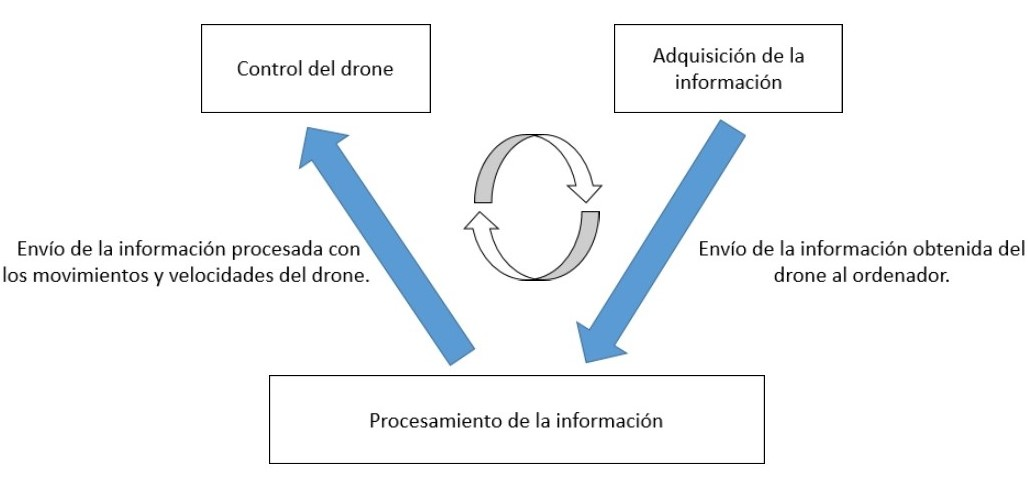
\includegraphics[width=0.75\textwidth]{imgs/esquema_d.jpg}
	\label{fig:esquema_d}
\end{figure}


\section{Percepci\'on.}
\hspace{1cm} En este apartado se tratar\'a sobre el procesamiento de la imagen obtenida. Este puede ser el punto mas importante de todos, pues es gracias al cual el drone sabe en que punto del algoritmo se encuentra y que informaci\'on enviar. Las primeras pruebas no eran muy complejas, obten\'iamos una imagen RGB que era la que se transmit\'ia, la convert\'iamos a HSV para que fuera mas f\'acil su interpretaci\'on, debido a que no tenemos tres colores a los que tratar sino tres parametros( Matiz, saturac\'on y valor). Lo que se consegu\'ia con esto era que un color no dependiera tanto de las condiciones del medio, pues variando poco los valores H y S no hay una gran modificaci\'on en el tono, y por lo tanto la intensidad de la luz influir\'a de menor manera. Tras esto se realiza un filtro de color, eligiendo los valores de H,S y V entre 0 y 255, quedandonos solo con los objetos que nos inter\'esaban. Una vez est\'abamos en este punto, si se trataba de una imagen perfecta, como pueden ser alg\'unas de simulador no hab\'ia problemas, pero en caso contrario, debido a factores como luces, sombras y reflejos, un color pod\'ia tratarse de distinta forma seg\'un el momento o que pasaran el filtro puntos de la imagen que no eran de las caracter\'isticas deseadas. Por ello,  era necesario el uso de operadores morfol\'ogicos, los cuales explico brevemente para que as\'i se entienda su uso: 
\begin{itemize}
	\item \textbf{Erosi\'on:} Dada una imagen y un elemento estructural, la erosi\'on es el conjunto de los elementos \textit{x} para los cuales el elemento estructural trasladado por \textit{x} est\'a contenido en la imagen. 
	\newline\hspace{1 cm} Aplicaci\'on: Cuando un p\'ixel que parece pasar el filtro, pero los elementos de su alrededor(en concordancia con el elemento estructurante) no lo pasan, este pasa a ser parte del fondo. 
	\item \textbf{Dilataci\'on:} Transformaci\'on dual a la erosi\'on. El resultado de esta es el conjunto de elementos tal que al menos alg\'un elemento del conjunto estructurante esta contenido en \textit{x}, cuando el elemento estructurante se desplaza sobre \textit{x}
	\newline\hspace{1 cm} Aplicaci\'on: p\'ixeles que parecen de fondo, pasan a ser de la figura si estan cerca de p\'ixeles que pasan el filtro.
	\item \textbf{Cierre:} Se trata de realizar una dilataci\'on en la imagen seguida de una erosi\'on.
	\item \textbf{Apertura:} Se trata de realizar la erosi\'on en una imagen seguido de la dilataci\'on.
\end{itemize}

\hspace{1cm} Pues bien, gracias a esto se puede hacer un pre-procesado de la imagen(t\'ecnica mediante la cual se mejoran y realzan las caracter\'isticas de esta para as\'i f\'acilitar las posteriores operaciones a realizar) y as\'i obtener una mejor imagen con la que trabajar. Hay que destacar que las mas utilizadas durante la realizaci\'on de este trabajo han sido la erosion y la apertura. Pues con la erosi\'on evit\'abamos que se colaran p\'ixeles de fondo como parte del objeto, por lo que obten\'iamos solo la parte requerida, y por otro lado con la dilataci\'on realizada en la apertura, tras eliminar el ruido de fondo, si en alg\'un objeto se quedaba un p\'ixel en negro consegu\'iamos que este pasara a formar parte de la figura, por lo que con estos metodos hab\'iamos conseguido el objetivo: eliminar el ruido de fondo y obtener el objeto de forma mas compacta.En la siguiente imagen podemos observar un ejemplo de esto:

\begin{figure}[ht]
	\centering
		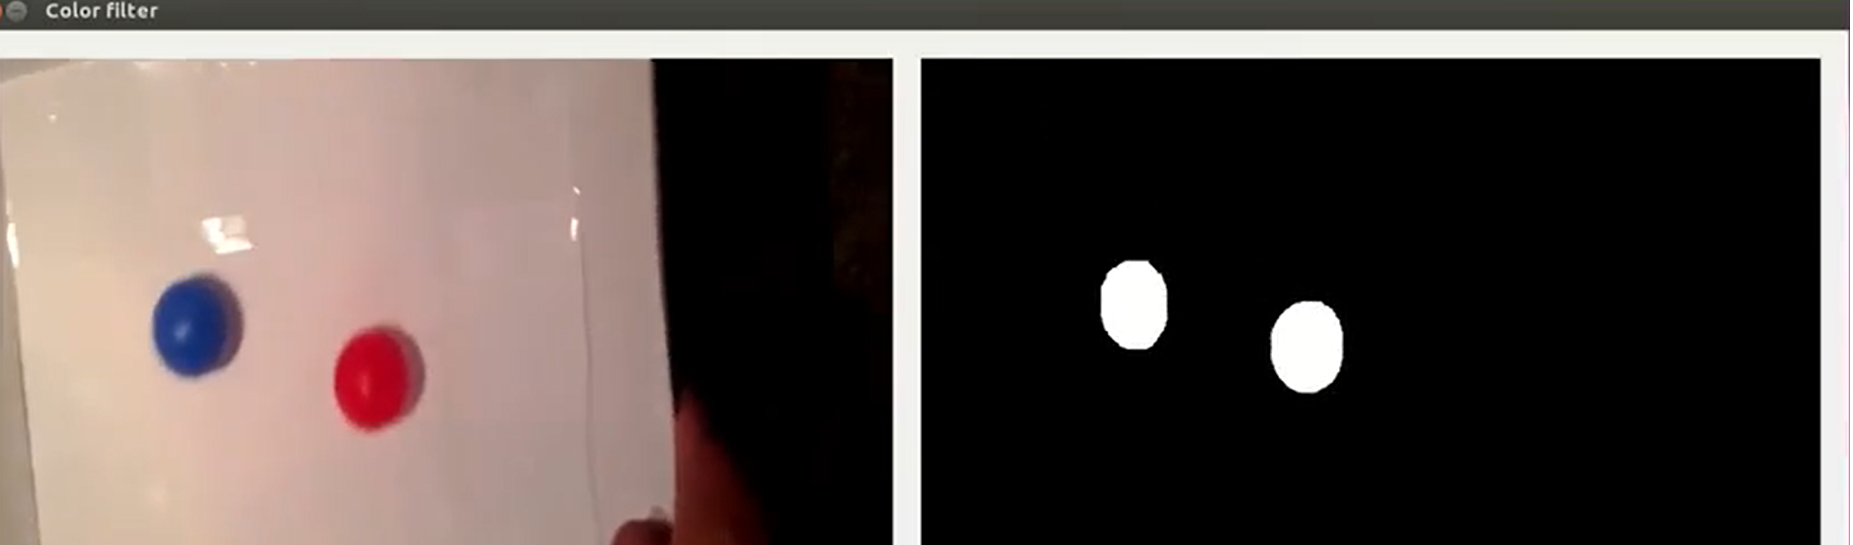
\includegraphics[width=1.0\textwidth]{imgs/colorfilter.eps}
		\caption{Esta imagen muestra un primer filtro de color.}
	\label{fig:ColorFilter}
\end{figure}

\hspace{1cm} A continuaci\'on pongo como ejemplo una parte de c\'odigo, el cual coge una imagen, la convierte a HSV, crea un filtro de color y pasa la imagen a trav\'es de este, obteniendo una imagen resultante:
\begin{verbatim}
hsv = cv2.cvtColor(input_image, cv2.COLOR_BGR2HSV)
lower_orange = np.array([100,100,80], dtype=np.uint8)
upper_orange = np.array([150, 255,255], dtype=np.uint8)
maskOrange = cv2.inRange(hsv, lower_orange, upper_orange)
maskRGBOrange = cv2.bitwise_and(input_image,input_image, mask= maskOrange)
\end{verbatim}
\hspace{1 cm} Destacar que con la \'ultima linea de este c\'odigo, conseguiriamos que la imagen resultante no quedara en blanco y negro, sino que lo objetos que pasan el filtro se mostraran en su color original. 

\hspace{1 cm} Con esto se obtuvo una primera buena señal, y era que sobre im\'agenes reales(con imperfecciones) consegu\'iamos realizar los filtros que queriamos, por lo que el siguiente paso fue decidir la forma que tendr\'ia la baliza y comenzar a trabajar en ella y sus caracter\'isticas. Esta baliza constaria de un cuadrado formado por 4 cuadrados de dos colores: 

\begin{figure}[ht]
	\centering
		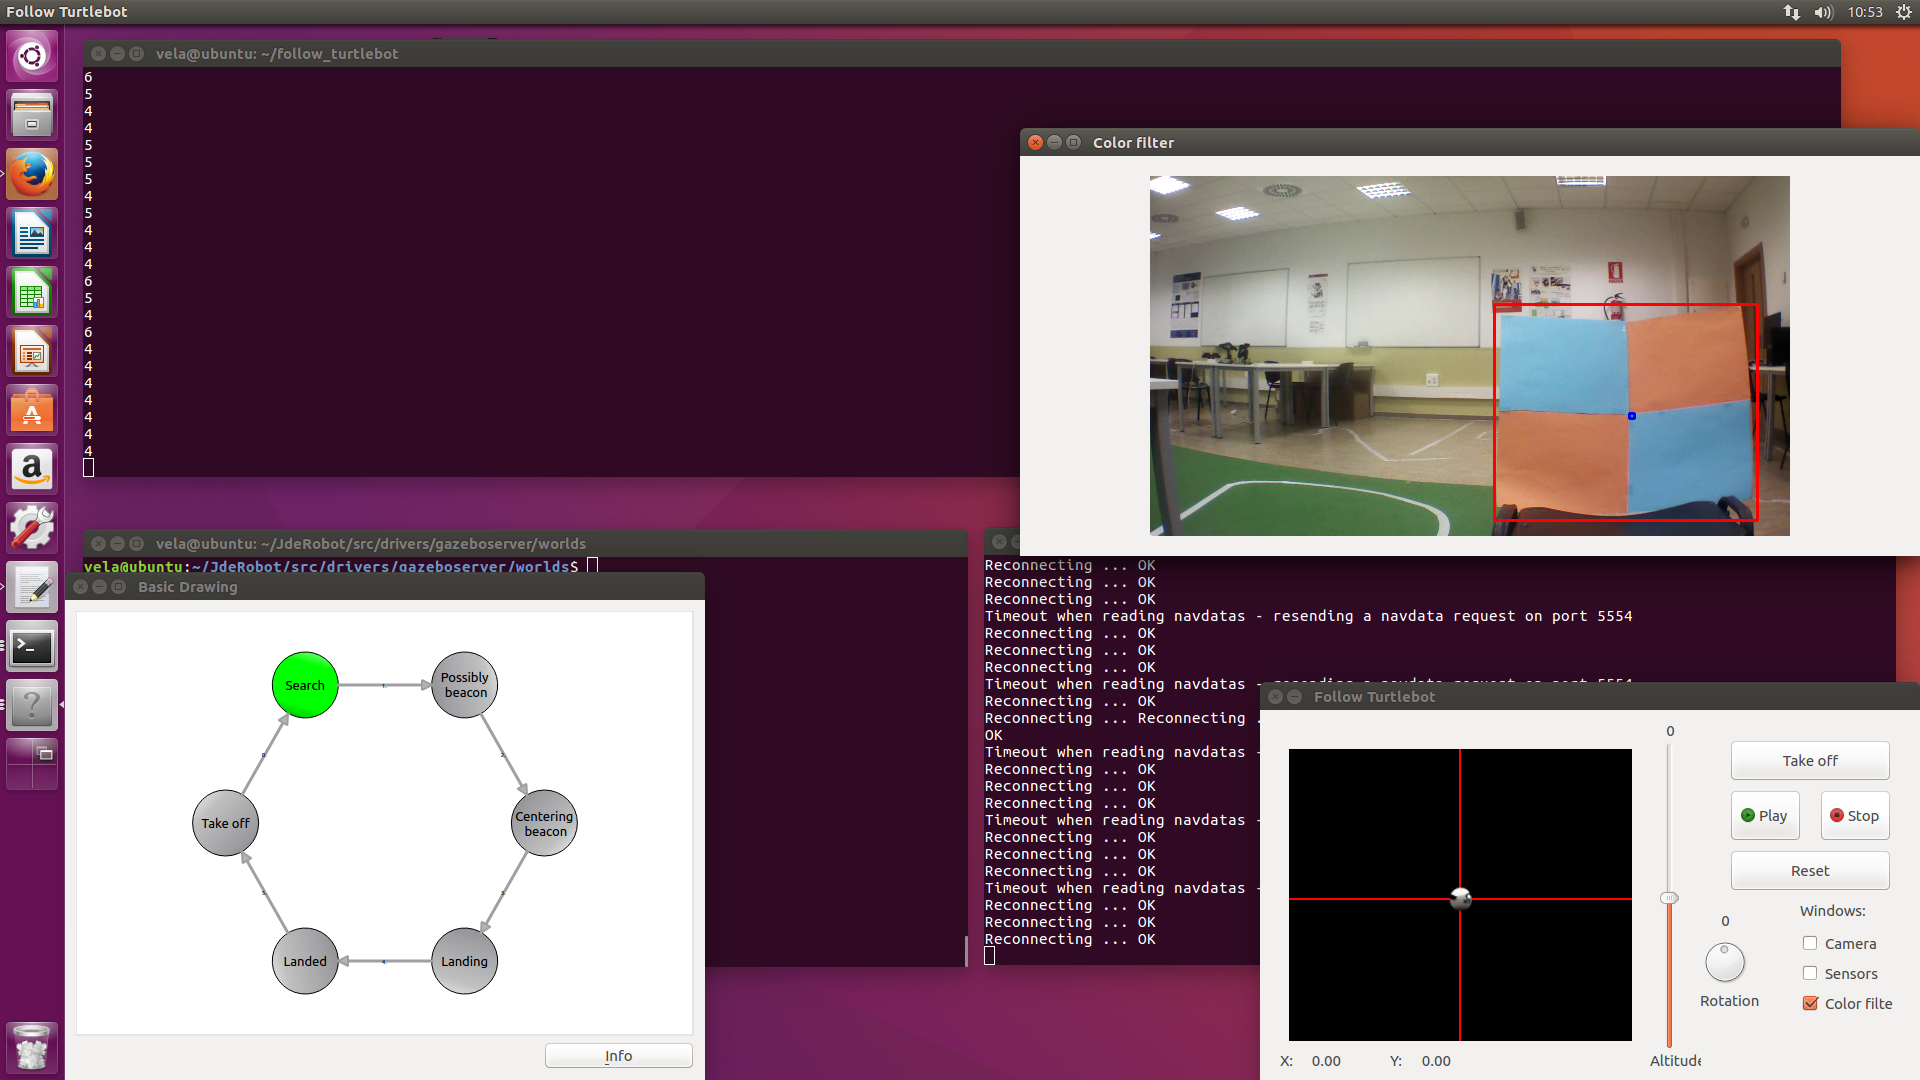
\includegraphics[width=0.4\textwidth]{imgs/k_beacon2.eps}
		\caption{Esta imagen muestra el conjunto de herramientas utilizadas.}
	\label{fig:Herramientas}
\end{figure}

\hspace{1 cm} Con la imagen de simulador, lo que tuvimos que hacer fue cambiar los valores al filtro de color anterior, con lo que ya consegu\'iamos obtener los colores de la baliza, pero sobre la baliza real se estuvo mas tiempo trabajando, pues al trabajar con ella en distintos entornos hab\'ia muchos cambios de luminosidad, y aunque HSV minimizara este problema, seg\'un el entorno de trabajo segu\'ia dando problemas. Al final ampliando el rango de colores, un mejor pre-procesado de esta imagen y el procesado para el algoritmo, se consigui\'o que esto no fuera un problema. 

\hspace{1 cm} Pero en realidad en este punto solo ten\'iamos el primer paso, que la baliza pasara el filtro de color, ahora ten\'iamos que conseguir que nuestro algoritmo detectara eso como una baliza para poder posicionarse sobre ella. Para este punto, se ha pasado por distintos puntos y algoritmos, los cuales se han ido mejorando o cambiando seg\'un los fallos que se ve\'ian, hasta llegar a un algoritmo final.

\hspace{1 cm} Lo primero que hicimos fue sobre el simulador. Se obten\'ia la posici\'on de los p\'ixeles donde se encontraba el objeto que pasaba el filtro, y a partir de esto se calculaba su p\'ixel central. Esto se hacia gracias a una funci\'on de OpenCV que retornaba el \'area que no se consideraba fondo, y luego de este \'area calculaba su centro. Un ejemplo del c\'odigo python que realiza esto, a partir del c\'odigo anterior, es el siguiente:

\begin{verbatim}
momentsOrange = cv2.moments(maskOrange)
x_center = int(momentsTot['m10']/momentsTot['m00'])
y_center = int(momentsTot['m01']/momentsTot['m00'])
\end{verbatim}

\hspace{1cm} Una vez hemos obtenido el centro del objeto, hay que calcular el centro de la imagen. En este caso, para calcularlo, hemos hecho es que la primera vez que se ejecute nuestro algoritmo(teniendo en cuenta que \'este est\'a en una continua ejecuci\'on) llame a una funci\'on a la que se le pasa la imagen de entrada, obtiene su tamaño y calcule a partir de este cual es el centro de la imagen. La raz\'on de hacer esto es que tanto el drone real como el del simulador tienen dos c\'amaras, que obtienen distintas im\'agenes con distintos tamaños, de esta forma se calcula el tamaño la imagen que se va a utilizar de manera autom\'atica antes de comenzar cualquier proceso. Pues bien, para hacer las pruebas iniciales, teniendo el centro de la imagen y el centro del punto al que queremos llegar, basta con hacer la resta de estos y multiplicarlos por un valor(en funci\'on de las velocidades del drone) para que este se mueva, centrando su centro y el del objeto. 

\hspace{1cm} Tras conseguir, con un filtro y unas funci\'ones, que el drone pudiera situarse sobre un objeto filtrado, pasamos a mejorar la detecci\'on de la baliza. La idea principal de la detecci\'on es detectar donde esta la cruz que forman los 4 cuadrados de colores, o lo que es lo mismo, detectar la intersecci\'on de los cuadrados de la baliza, as\'i obtendremos el punto sobre el cual situarnos para podernos centrar. 

\hspace{1cm} Un primer algoritmo fue realizar los dos filtros de color, uno por cada color de la baliza, obteniendo as\'i por separado los colores verde y naranja cuando trabaj\'abamos en el simulador. Una vez obten\'iamos las im\'agenes por separado realizamos una dilataci\'on de ambas im\'agenes y luego una suma, lo que nos daba como resultado otra vez la baliza inicial pero con las intersecciones de otro color, de forma que filtrando por este nuevo color obtenido obten\'iamos la cruceta de la baliza. En este punto en el \textit{color filter} de la herramienta ve\'iamos los dos filtros por separado y la intersecci\'on de ambos:

\begin{figure}[ht]
	\centering
		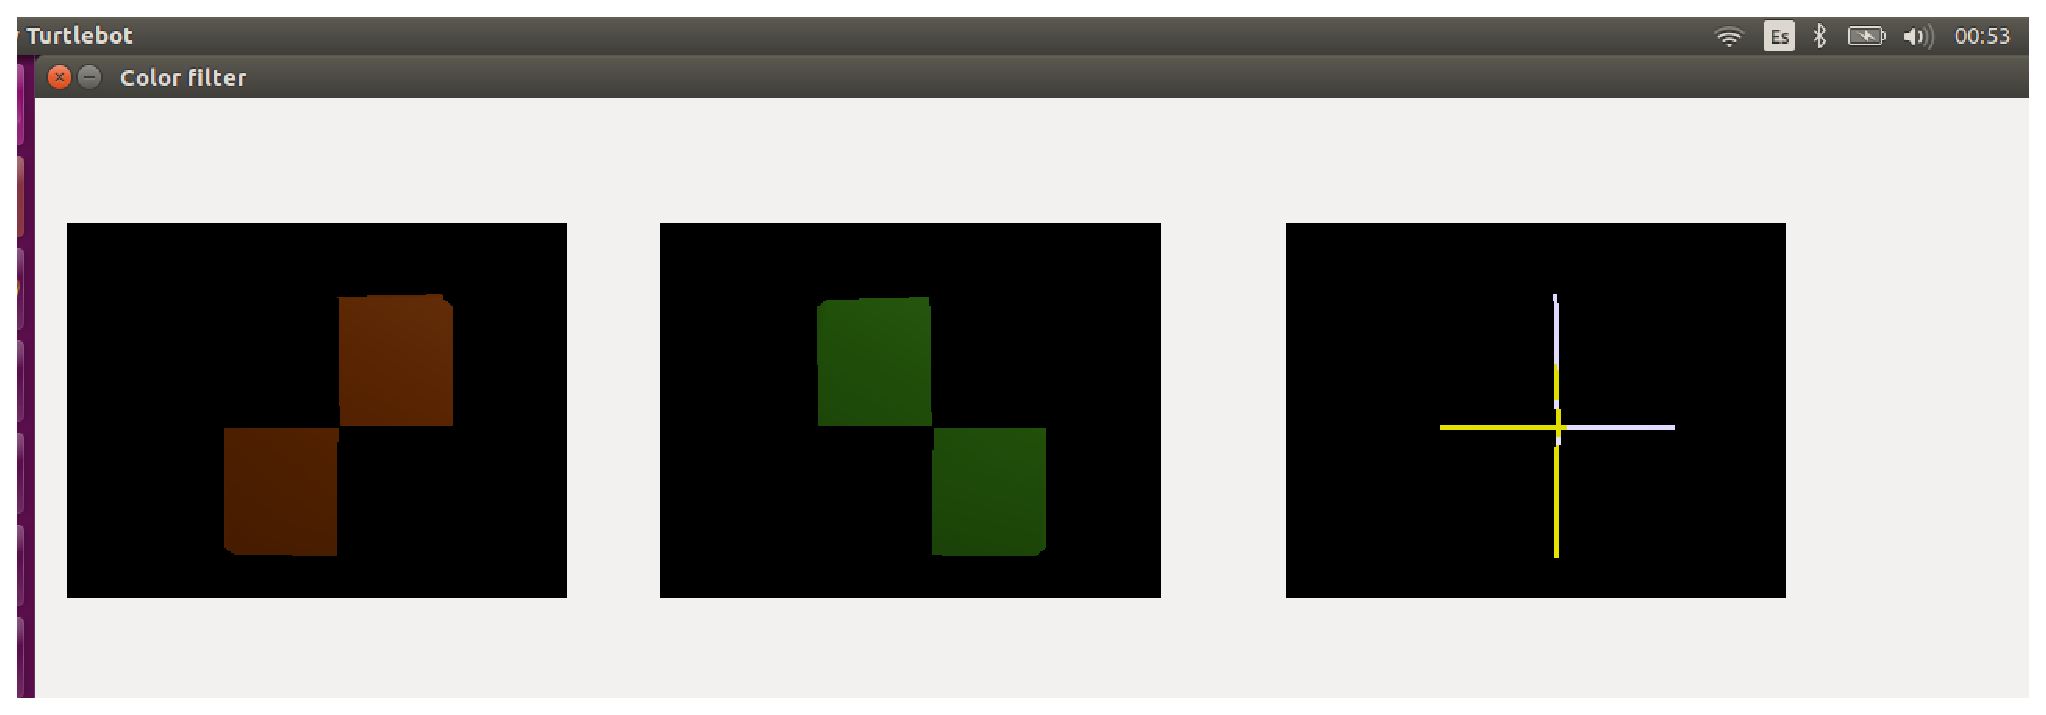
\includegraphics[width=0.8\textwidth]{imgs/E_Imagen_baliza.eps}
	\label{fig:E_Imagen_baliza}
\end{figure}

\hspace{1cm} En este punto, cuando el drone detectaba un objeto en la figura de la izquierda, lo trataba como baliza, por tener los dos colores principales juntos, pero aun quedaba mucho camino por recorrer, pues no detect\'abamos el centro de la intersecci\'on. Por otro lado, fue en este punto donde decidimos que las ventanas que mostraba el \textit{color filter} ya no era tan necesaria, pues hab\'iamos obtenido lo que queriamos, y se decidi\'o trabajar hacia una ventana que mostrara la imagen completa de lo que estaba viendo el drone y marcara de alg\'una forma el contorno y cruceta de dicha baliza. Para esto fueron muy \'utiles las funci\'ones \textit{findContours} y \textit{drawcontours} de OpenCV, las cuales nos permit\'ian encontrar los bordes de los objetos de las im\'agenes y marcar estos. Lo que hac\'iamos en este proceso era obtener los bordes de las im\'agenes que hab\'ian pasado el filtro y despues pintar sobre la imagen original.Para poder utilizar esta funci\'on necesit\'abamos pasar la imagen a escala de grises, como podemos ver a continuaci\'on:

\begin{verbatim}
imgray1 = cv2.cvtColor(maskRGBOrange,cv2.COLOR_BGR2GRAY)
ret,thresh = cv2.threshold(imgray1,255,255,255)
_,contours, hierarchy = cv2.findContours(thresh,cv2.RETR_TREE,cv2.CHAIN_APPROX_SIMPLE)
cv2.drawContours(input_image, contours, -1, (0,255,0), 5)
\end{verbatim}

\hspace{1cm}Conseguido esto, para el simulador ten\'iamos un algoritmo principal que hac\'ia lo que busc\'abamos en situaciones ideales, pero segu\'ia teniendo varios fallos.
\hspace{1cm} El primero a arreglar era que si en lugar de 4 cuadrados la baliza solo tenia dos, al dilatar y filtrar obtendr\'iamos de igual forma otra figura, aunque en lugar de una cruceta se tratara de una linea. La forma de enfrentarse a esto fue contando el numero de objetos que hab\'ia en la imagen. Si la imagen ten\'ia dos objetos de cada color y un objeto que fuera la intersecci\'on de los otros, se tratar\'ia de una baliza, en caso de no ser de esta forma no se tratar\'ia como tal. En la parte de visi\'on estuvimos mucho tiempo trabajando con este algoritmo, pues para el simulador funci\'onaba bien. Pero en este punto, en la parte de visi\'on, detecci\'on de colores y realizaci\'on del filtro, comenzamos a trabajar con el drone real, haciendo tareas muy simples, por lo que mejorar la robustez de esto se quedo un poco de lado. 

\hspace{1cm} Para comenzar a probar el filtro de colores en el drone real se hizo una baliza como la que ten\'iamos en el simulador, pero al ir a realizar las primeras pruebas estaba el problema de que en la realidad hab\'ia muchos colores parecidos en las distintas direcciones, por lo tanto el drone confund\'ia muy f\'acil los colores. Para arreglar esto se empez\'o trabajando sobre un color y mejorando el algoritmo, de tal manera que el rango de colores fuera mas reducido, y aunque esto era un problema porque al trabajar con la luz real, un mismo color variaba mucho su rango seg\'un  la situaci\'on que estuviera, trabajando en HSV se consigui\'o, y tras esto en el pre-procesado se realiz\'o una erosi\'on con mas iteraciones de forma que eliminaba mejor los p\'ixeles de fondo, pues en estas pruebas el problema era que uno de los colores de fondo era muy parecido al color de la cartulina. Tambi\'en añadimos que el drone solo hiciera caso a los objetos con un \'area mayor a determinado valor, con lo que consegu\'iamos que si alg\'un objeto de fondo segu\'ia pasando el filtro lo obviara.

\hspace{1cm} Despues de esto ya quedaba la ultima parte por parte del filtro de colores aunque la mas dificil: \textit{conseguir situar una baliza en condiciones reales}. La primera complicaci\'on de esto es el detectar dos colores muy distintos, el problema de esto era que en cualquier entorno que estuvieramos era muy probable tener de fondo un color muy parecido a cualquiera de los dos, pero como anteriormente, fue reforzar el filtro y pre-procesado para conseguir esto. Una vez conseguimos las pruebas eran sencillas: hacer despegar al drone y poner la baliza delante. Una vez que movieramos la baliza el drone deb\'ia moverse en el mismo sentido, prueba que, aunque costosa, se realizo con \'exito. Destacar que tambi\'en en este momento la imagen que mostraba \textit{color filter} se volvi\'o a modificar, pues se mostraba la imagen real y sobre ella se pintaba, si era posible baliza, los bordes y la cruceta en verde. En el momento que se trataba de la baliza real, los bordes se pintaban en rojo (valor RGB 255,0,0) y la cruceta en verde (valor RGB 0,255,0). De esta forma era muy f\'acil saber, con solo visualizar la imagen, en que punto se encontraba el algoritmo y si actuaba correctamente.


\hspace{1cm} Ya con un algoritmo de detecci\'on con el que se pod\'ia trabajar correctamente, todav\'ia le faltaba algo de robustez, pues si situ\'abamos un objeto del mismo color que alg\'uno de los colres de la baliza lo detectaba como un objeto mas, lo que llevaba a que el numero de objetos de un color fuera mayor, y daba problemas como el que el n\'umero de objetos de un color fuera mayor, el \'area era mayor que el deseado y en caso de calcular el centro del \'area no lo situaba donde deb\'ia. Por lo tanto, se llego a una soluci\'on que, aunque tardaba mas en procesar la imagen, es mas robusta. El proceso es el siguiente:
\begin{enumerate}
	\item Como anteriormente, pasar los filtros de color y obtener solo los objetos de los colores deseados, pasando el resto a ser p\'ixeles de fondo. De Aqu\'i obtenemos dos im\'agenes, una por color.
	\item De cada imagen, obtenemos el n\'umero de objetos, sus \'areas y sus contornos. Vamos recorriendo los objetos de las im\'agenes,  en caso de tener un \'area mayor a un valor determinado, se crea una imagen negra del mismo tamaño que la imagen de entrada, y se pinta sobre esta el contorno del objeto con un valor determinado, ponamos como ejemplo que cada contorno tiene un valor RGB (0,1,0). De forma que, si por ejemplo, el numero de objetos tras pasar los dos filtros era 5, obtendremos 5 im\'agenes. 
	\item Por cada imagen obtenida, dilatamos lo obtenido(por lo que el borde se ensanchara) y lo sumamos a una imagen final, de forma que en cada imagen, donde se sit\'ue el contorno se sumara a cada p\'ixel un valor RGB(0,1,0). De forma que el punto que sea la intersecci\'on de dos objetos, el valor sera(0,2,0) y donde sea la intersecci\'on de 4 objetos el valor sera (0,4,0). El punto donde interseccionen 4 objetos ser\'a la cruceta (ejemplo de la suma de im\'agenes en figura 4).
	\item Una vez tenemos esta im\'agen final, le podemos aplicar un filtro RGB que permita pasar los p\'ixeles con valor (0,4,0), de forma que de la cruceta solo obtendremos el punto donde interseccionan los 4 cuadrados.
	\item Ya con la imagen que solo muestra los p\'ixeles de intersecci\'on, podemos utilizar la funci\'on drawcontours, que a parte de permitirnos marcar el centro sobre la imagen original, nos retorna el valor de los p\'ixeles que pinta, de donde obteniendo su centro, podemos obtener con exactitud los valores X e Y donde se situa la cruceta.
	%\item Ya teniendo este valor, por otro lado hemos continuado con la realizaci\'on de otro filtro, el cual pinta de verde los bordes de los objetos sobre la imagen original, miramos si el valor (X,Y) obtenido en el filtro anterior coincide con un valor pintado en esta imagen. En caso de coincidir podemos asegurar que e trata del centro de la baliza.
	\item Para finalizar este proceso, se realizo de nuevo un cambio en \textit{color filter}, en el cual con la funci\'on rectangle de OpenCV marcamos la cruceta de la baliza(como se puede ver en la figura dos de la p\'agina 17) y con un cuadrado rojo los objetos que son posibles balizas, marcando de esta forma la baliza real.
\end{enumerate}
\vspace{2mm}
\begin{figure}[ht]
	\centering
		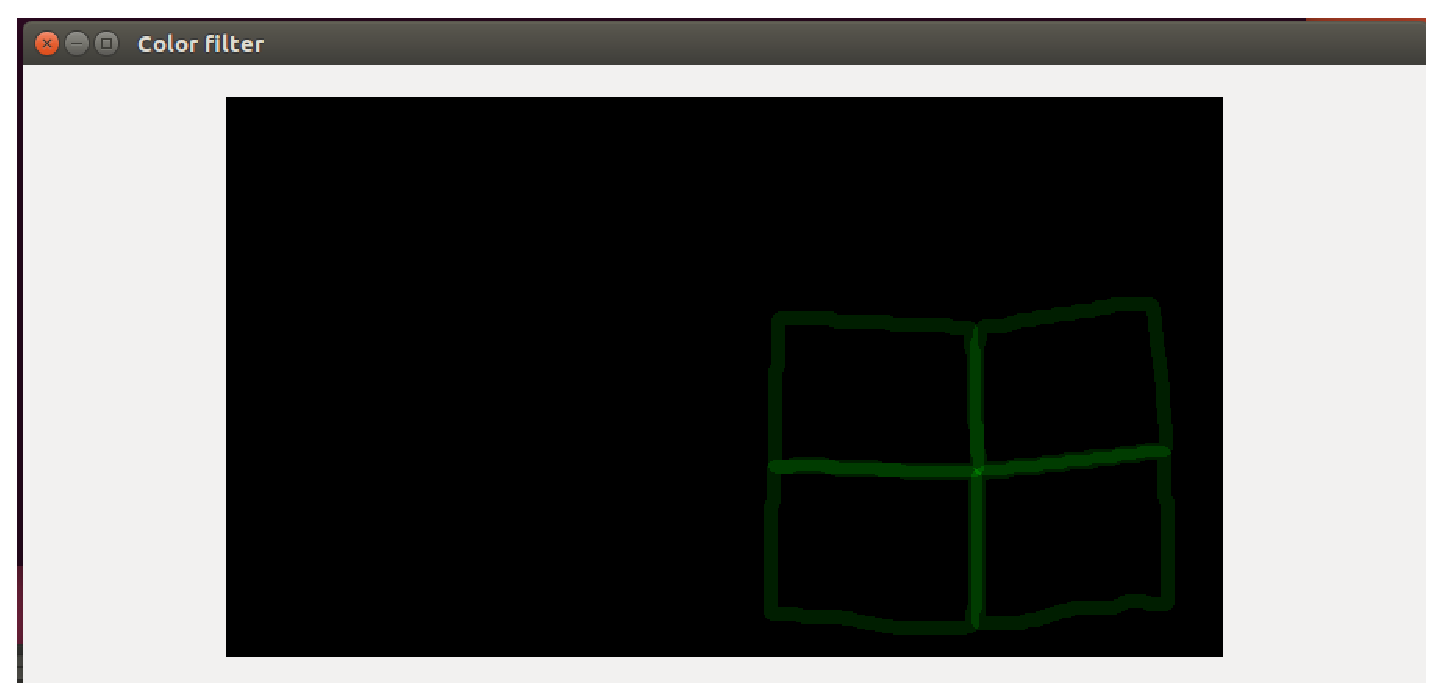
\includegraphics[width=1.1\textwidth]{imgs/k_Beacon1.eps}
		\caption{Imagen que muestra la suma de las diferentes im\'agenes creadas por cada objeto.}
	\label{fig:k_Beacon1}
\end{figure}
\vspace{3mm}

\hspace{1cm} A continuaci\'on inserto un fragmento de c\'odigo, el cual a partir de una imagen que ha pasado un filtro, pinta los contornos de cada objeto, cada uno sobre una nueva imagen negra, y las guarda en un array. Tras esto dilata y suma las im\'agenes obteniendo la imagen final.

\begin{verbatim}
f = []
i=0
imgray2 = cv2.cvtColor(maskRGBOrange,cv2.COLOR_BGR2GRAY)
ret,thresh = cv2.threshold(imgray2,255,255,255)
_,contours, hierarchy = cv2.findContours(thresh,cv2.RETR_TREE,cv2.CHAIN_APPROX_SIMPLE)
\'areas = [cv2.contour\'area(c) for c in contours]
for extension in \'areas:
    if extension > 100:
    img = np.zeros((y_img*2,x_img*2,3), np.uint8)
        actual = contours[i]
        approx = cv2.approxPolyDP(actual,0.05*cv2.arcLength(actual,True),True)
        cv2.drawContours(img,[actual],0,(0,30,0),12)
        f.append(img)
        i=i+1
			
kernel = np.ones((3,3),np.uint8)
if(len(f)>0):
    f[0] = cv2.dilate(f[0],kernel,iterations = 4)
    show_image2=f[0]
    for k in range(len(f)-1):
        f[k+1] = cv2.dilate(f[k+1],kernel,iterations = 4)
        show_image2=show_image2+f[k+1]
		
\end{verbatim}

\hspace{1cm} Por otro lado, voy a mostrar un fragmento de c\'odigo en el cual, a partir de la imagen que muestra el borde de la baliza, la cruceta y el centro en determinados valores, obtengo los p\'ixeles sobre los que se centra la cruceta. La raz\'on de que se inicien a un valor negativo es para que al retornar estos valores cuando se llama a la funci\'on, el algoritmo sepa que no se ha detectado la intersecci\'on entre los cuatro cuadrados de la baliza. 


\begin{verbatim}
lower_green = np.array([0,80,0], dtype=np.uint8) 
upper_green = np.array([0, 255,0], dtype=np.uint8) 
maskSHI = cv2.inRange(show_image2, lower_green, upper_green)
show_image2 = cv2.bitwise_and(show_image2,show_image2, mask= maskSHI)

compare_image = np.zeros((y_img*2,x_img*2,3), np.uint8)
diff_total = cv2.absdiff(compare_image, show_image2)

imagen_gris = cv2.cvtColor(diff_total, cv2.COLOR_BGR2GRAY)
_,contours,_ = cv2.findContours(imagen_gris,cv2.RETR_EXTERNAL,cv2.CHAIN_APPROX_SIMPLE)

positionX=-1
positionY=-1
for c in contours:
    if(cv2.contour\'area(c) >= 0):
        posicion_x,posicion_y,ancho,alto = cv2.boundingRect(c) 
        cv2.rectangle(show_image,(posicion_x,posicion_y),(posicion_x+ancho,posicion_y+alto)
        ,(0,0,255),2)
        positionX= (posicion_x+posicion_x+ancho)/2
        positionY= (posicion_y+posicion_y+ancho)/2
\end{verbatim}

\section{Control.}
\hspace{1cm} Una vez terminado el filtro de color, hablemos del algoritmo de movimiento del drone. Las primeras pruebas sobre simulador se realizaban de forma simple: El drone despegaba, y mientras no detectara baliza sobre la que centrarse, sub\'ia dando vueltas sobre si mismo, en el momento que encontraba la baliza obten\'ia el centro de esta e intentaba que coincidiera con el centro de la imagen. Tras esto se probo que la baliza se desplazara y que el drone fuera capaz de seguirla. Prueba que tambi\'en funci\'ono sin problemas. Al depender la velocidad de la resta de los centros, provocaba que al estar mas lejos la velocidad de movimiento fuera mayor y fuera disminuyendo conforme se centraba, evitando de esta forma que el drone frenara de forma brusca y disminuir los balanceos y turbulencias. 
Aun as\'i, se detectaban ciertas imperfecciones debido a que se trataba de un controlador proporcional, el cual funci\'onaba bien pero no lo suficiente, por lo que se decidi\'o añadir una componente derivativa, con el objetivo de mantener el error al m\'inimo, evitando que este se incremente y por lo tanto el drone sufra cada vez mas oscilaciones al situarse sobre un punto. Este control se basa en derivar el error con respecto al tiempo y multiplicarlo por una constante. Dado que nuestro algoritmo ejecuta una vez cada cierto tiempo y no esta continuamente pasando por este punto, podemos considerar que se trata de un sistema en tiempo discreto, y por tanto en lugar de trabajar con derivadas trabajaremos con sumatorios. De esta forma, para añadir un control derivativo realiz\'abamos una operaci\'on que depende de la velocidad anterior y la que tenemos ahora: \[v_{derivativa} =1-(v_{anterior}-v_{nueva})/50 \]  
\hspace{1cm} En nuestro algoritmo, en caso de que la operaci\'on de un valor menor a 0.1 lo igualamos a este, con lo que conseguimos que nunca sea un valor muy cercano a 0 y por lo tanto no se quede en el sitio. Este resultado lo multiplicamos a la velocidad final, y lo que conseguimos es que si el valor entre dos velocidades continuas es muy alto este se aten\'ue de forma que el drone no cambie mucho y vaya oscilando, sino que lleve una velocidad mas continua, de cara a acelerar o frenar su velocidad. 

\hspace{1cm} Por otro lado, el drone tiene un algoritmo de b\'usqueda, en el que se pretende que se mueva realizando una espiral continua, haciendo as\'i que recorra toda la zona de su alrededor. Para ello se le env\'ia la informaci\'on de dos velocidades que fueran variando con el paso de las iteraciones, una que depend\'ia de la rotaci\'on sobre si mismo, y otra velocidad que se le pasaba para que hiciera en su eje X hacia delante. De esta forma, con el paso de las iteraciones disminu\'ia la velocidad de rotaci\'on, al mismo tiempo que aumentaba la velocidad hacia delante, con lo que consegu\'iamos un algoritmo de busqeda en espiral, pudiendo recorrer de esta forma un determinado \'area con f\'acilidad. Un ejemplo de esto lo podemos ver en el siguiente fragmento de c\'odigo.

\begin{verbatim}
self.cmdvel.sendCMDVel(1.8+wSearch,0,0,0,0,1.5 - wSearch)
numVuelta=numVuelta+1
if(numVuelta==100):
    timerW=timerW+(timerW/8)
    numVuelta=0
    if(wSearch<1):
        wSearch=wSearch+0.2
\end{verbatim}

\hspace{1cm}	

\hspace{1cm} Para poder añadirlo lo unico que se tuvo que hacer es añadir dos paquetes del GUI de JdeRobot, uno que permitia abrir otra ventana y otro que permitia añadir estados y transiciones entre ellos. Para marcarlo, siendo el numero que aparece el numero del estado que queremos marcar, val\'ia con la siguiente linea de c\'odigo:

\begin{verbatim}
self.machine.setStateActive(2, True)
\end{verbatim}
	
Visualmente, durante la ejecuci\'on obten\'iamos esto:
\begin{figure}[ht]
	\centering
		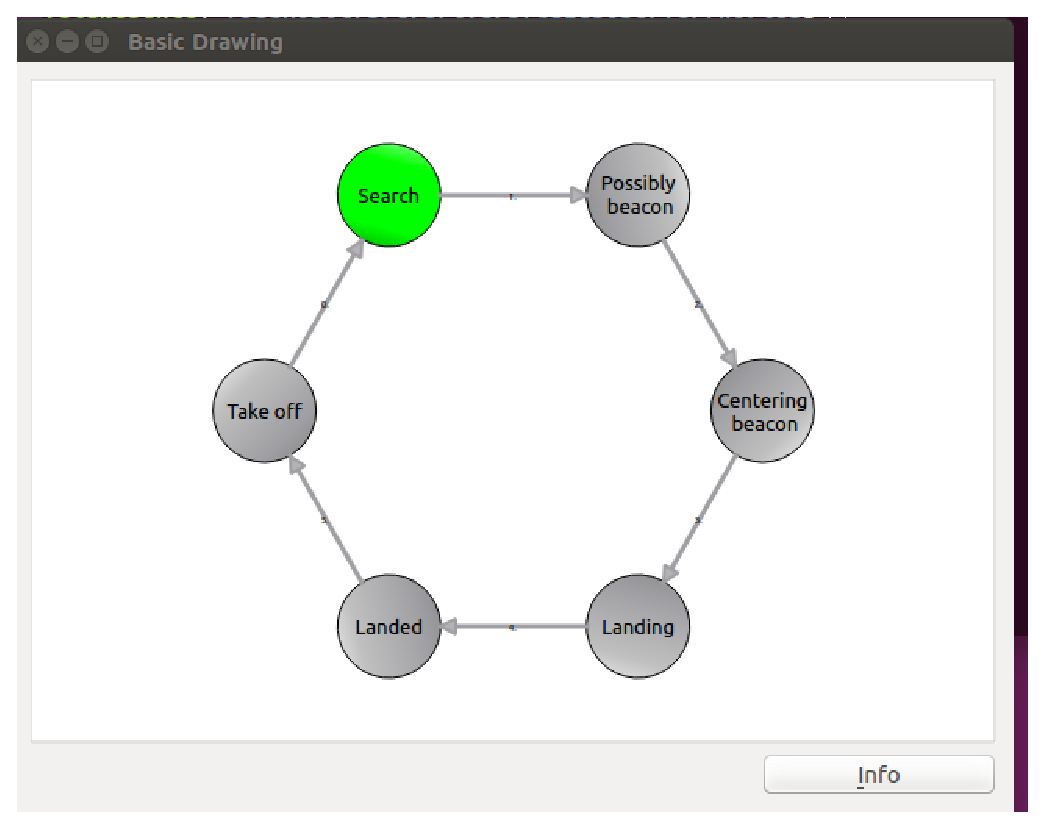
\includegraphics[width=0.3\textwidth]{imgs/states.eps}
		\caption{Imagen que muestra el diagrama de estados.}
	\label{fig:k_Beacon1}
\end{figure}

\section{funci\'onamiento del algoritmo.}
\hspace{1cm} En realidad, todo lo contado del algoritmo sirve para satisfacer estas tres partes. 

\hspace{1cm} \textbf{El despegue} del drone. Para estas pruebas se ha estimado que el despegue ser\'a un periodo de 10 segundos para que este pueda estabilizarse sobre la baliza. Aunque es la parte mas sencilla, en un principio pensamos que todo ocurrir\'ia en perfecta forma, sin embargo al comenzar a trabajar con el Ardrone nos dimos cuenta de que bien por las corrientes internas que se forma en espacios cerrados, o por la inestabilidad de este simplemente por el paso del tiempo y que su estructura ya no esta en como en un inicio, una vez en el aire no manten\'ia la posici\'on, sino que se desplazaba cuando se le enviaban instrucciones de quedarse en el sitio(en mi caso,con el drone que trabajaba una vez se levantaba comenzaba a ir hacia atr\'as). Debido a esto, decidimos que el despegue se controlara tambi\'en mediante visi\'on. Lo que pretend\'iamos con esto es que una vez el drone estuviera en el aire, detectara una baliza de color naranja, calculara su centro e intentara situarse sobre este, asegurandonos as\'i realmente que el drone permanec\'ia en el sitio. Trabajando en \'esta idea nos dimos cuenta que el drone ten\'ia un par de segundos en el despegue en los que trabajaba de forma autom\'atica y no es capaz de realizar las acciones que se le est\'an enviando, lo que lleva a estar los dos segundos iniciales sin control sobre este. Durante este periodo se marca el estado "`Take off"' en el diagrama de estados.

\hspace{1cm} Una vez tenemos el drone en el aire llegamos a la parte mas compleja, \textbf{la b\'usqueda} de la baliza. En este momento se marca el estado "`Search"' en el diagrama de estados, y el drone comienza a moverse en forma de espiral mientras busca alg\'un objeto que tenga los colores de la baliza. En el momento que encuentra uno de los dos colores marca el estado "`Possibly beacon"' e intenta centrarse sobre el objeto, esperando que se trate de una baliza. En caso de no tratarse de la baliza, el drone se aparta de esta y continua con su algoritmo de b\'usqueda, pero en caso de serlo marca sobre el diagrama de estados "`Centering beacon"' haciendo que coincidan sus centros. Aqu\'i ya no se fija en el \'area del objeto como en el caso anterior, para centrarse sobre el centro de este, sino que al haber obtenido ya donde est\'a la cruceta, tiene sus valores desde un principio, por lo que es sobre estas coordenadas sobre las que tiene que situarse. Destacar que pueden darse factores externos por los cuales el drone pierda parte de la baliza y no la detecte como tal, pero si siga detectando objetos, en este caso tratara a tales objetos como la baliza e intentara situarse de nuevo sobre ellos durante un periodo de tiempo. En caso de tratarse de alg\'un otro factor y que ya no exista baliza en este punto continuara buscando. Una vez el centro de la imagen y la cruceta est\'an a una distancia menor de un determinado n\'umero de p\'ixeles, aparte de centrarse comienza su descenso, hasta que la baliza en la imagen tiene un determinado \'area en el que se considera que ya esta suficientemente cerca y deja de descender. 

\hspace{1cm} Es en este momento cuando comienza la parte del \textbf{aterrizaje}, esto se debe a que el aterrizaje en si tambi\'en es un proceso que se realiza un poco a ciegas, pues en el momento que env\'ias la instrucci\'on de "`land"' al drone este comienza a descender hasta que llega al suelo y para sus motores. Este momento se produce cuando el drone esta pr\'acticamente centrado sobre la baliza y a una distancia cercana, que nos podamos asegurar que en el periodo de aterrizaje no se va cruzar ning\'un obst\'aculo ni se van a producir accidentes. Se marca en el diagrama de estados "`Landing"' y el drone comienza a descender en vertical hasta encontrar el sitio donde posarse. Una vez aterrizado para sus motores y se marca el estado "`Landed"', habiendo finalizado de esta forma el algoritmo. 


